\documentclass[dvipdfmx,12pt]{beamer}
\usepackage{pxjahyper}
\usepackage{minijs}
\usepackage{amsmath}
\usepackage{fancybox}
\usepackage{array}
\usepackage{graphicx}
\usepackage{ascmac}
\usepackage{color}



\usetheme{Madrid}
\usecolortheme{default}
\renewcommand{\kanjifamilydefault}{\gtdefault}

\useoutertheme[subsection=false]{smoothbars}
\setbeamertemplate{footline}[page number]
\setbeamerfont{footline}{size=\small,series=\bfseries}
\setbeamercolor{footline}{fg=black,bg=black}






\title{最大の移動時間を最小化する教室割当問題の\\定式化と求解}
\author{\Large {システムモデリング研究室\\都11-0023 岡崎 俊介}}
\date{{\Large 2015年2月16日}}
\begin{document}

\begin{frame}\frametitle{}
\titlepage
\end{frame}

\begin{frame}                  %% \begin{frame}..\end{frame} で 1 枚のスライド
\titlepage{}                 %% タイトルページ
\end{frame}


\begin{frame}
  \frametitle{\LARGE 背景と定義}
\if0
\fbox{
\begin{tabular}{l|l}
{\Large \hspace{-3.0mm}背景}

& {\Large \hspace{-2.0mm}・関西大学の休み時間:10分}\\
& {\Large \hspace{-2.0mm}・休み時間内での移動が困難なことがある.}\\
\end{tabular}
}
\vspace{2.0mm}

\fbox{
\begin{tabular}{l|l}
{\Large \hspace{-3.0mm}定義}

& {\Large \hspace{-2.0mm}・各授業}\\
& {\Large \hspace{3.0mm}教室割当を行う.}\\

\end{tabular}
}
\fi
\begin{itembox}[c]{\Large{背景}}
\begin{center}
\begin{itemize}
\item{\large{関西大学では手動で教室割当を行っている.}}
\item{\large{関西大学の休み時間は10分と短い.}}
\item{\large{連続して授業をもつ学生は次の授業の移動と準備を時間内に行うことが困難なことがある.}}
\end{itemize}
\end{center}
\end{itembox}
\vspace{1.0mm}
\begin{itembox}[c]{\Large{移動時間を最小化する教室割当問題の定義}}
\begin{center}
\large{各授業の開講曜限が定められているとき,\\休み時間における全学生の移動時間の総和が\\最小となるような,授業に対する教室の割当を求めよ.}
\end{center}
\end{itembox}
\if0
\vspace{2.0mm}

\fbox{
\begin{tabular}{l|l}
{\Large \hspace{-3.0mm}手順}

& {\Large \hspace{-2.0mm}・最適化問題として教室割当問題を定式化}\\
& {\Large \hspace{-2.0mm}・定式化の際,2種類の制約を定める.}\\


 & {\Large \hspace{10.0mm}・絶対制約 - 必ず守るべき制約}\\
 &{\Large  \hspace{10.0mm}・考慮制約 - できるだけ守りたい制約}\\
\end{tabular}
}
\fi
\end{frame}


\begin{frame}
 \frametitle {\LARGE 手順}
\vspace{2.0mm}

\fbox{ 
\begin{tabular}{ll}
 {\LARGE 定式化}
\end{tabular}
}\\
%\vspace{2.0mm}
\begin{itemize}
\item{\Large{最適化問題として本問題を定式化}}
\item{\Large{定式化の際,2種類の制約を定める.}}
\begin{itemize}
\item{\Large{絶対制約:必ず守るべき制約}}
\item{\Large{考慮制約:できるだけ守りたい制約}}
\end{itemize}
\end{itemize}
\vspace{3.0mm}
\fbox{ 
\begin{tabular}{ll}
{\LARGE 移動時間の最小化}
\end{tabular}
}\\
%\begin{itemize}
%\item {\Large 総移動時間=(各教室間の移動時間\ ×\ 移動する人数)}\\
%\end{itemize}
\vspace{2.0mm}
{\Large 総移動時間=(各教室間の移動時間\ ×\ 移動する人数)の総和}

\end{frame}


\begin{frame}
  \frametitle{\LARGE 制約}
%	\Large{絶対制約}
\begin{itemize}
\item{絶対制約}
  \begin{enumerate}
  \item {\large 1つの曜限における各教室には2つ以上の\\授業を割り当てられない.}
  \item {\large 各授業には必ず1つの教室を割り当て\\なければならない.}
  \item {\large 受講人数が教室の定員を超えてはならない.}
  \item {\large 特定の授業は指定された教室で開講する.}
%  \item {\Large 移動時間は休み時間以内でなければならない.}
  \end{enumerate}
\item{考慮制約}
  \begin{enumerate}
  \item {\large 特別連続授業は同じ教室で開講されることが\\好ましい.}
	\begin{itemize}
	\item{\large{特別連続授業とは授業内容が同一,または非常に関連性の高い2限連続で開講される2つの授業}}
	\end{itemize}
  \item {\large 移動時間は指定した時間内であることが好ましい.}
  \item {\large 教室内の人が入れ替わる際の混雑ができるだけ\\ 発生しないほうが好ましい.}
  \end{enumerate}
\end{itemize}
\end{frame}

\begin{frame}
 \frametitle{\LARGE 絶対制約の例}

\fbox{ 
\begin{tabular}{ll}
{\Large 絶対制約1}
\end{tabular}
}\\
\begin{center}
{\Large 各教室:1つの授業が開講される or 空き教室}\\
\vspace{2.0mm}
{\Large $\displaystyle \sum_{j \in J}u_{i,j} \cdot e_{p,j} \leq 1$}
\hspace{1.0mm}
{\Large($i \in I,j \in J,p \in P$)}\\
\vspace{-2.0mm}
{\Large($i$:教室,$j$:授業,$p$:時限)}
\end{center}
\vspace{-4.0mm}
\begin{figure}[htbp]
 \begin{center}
  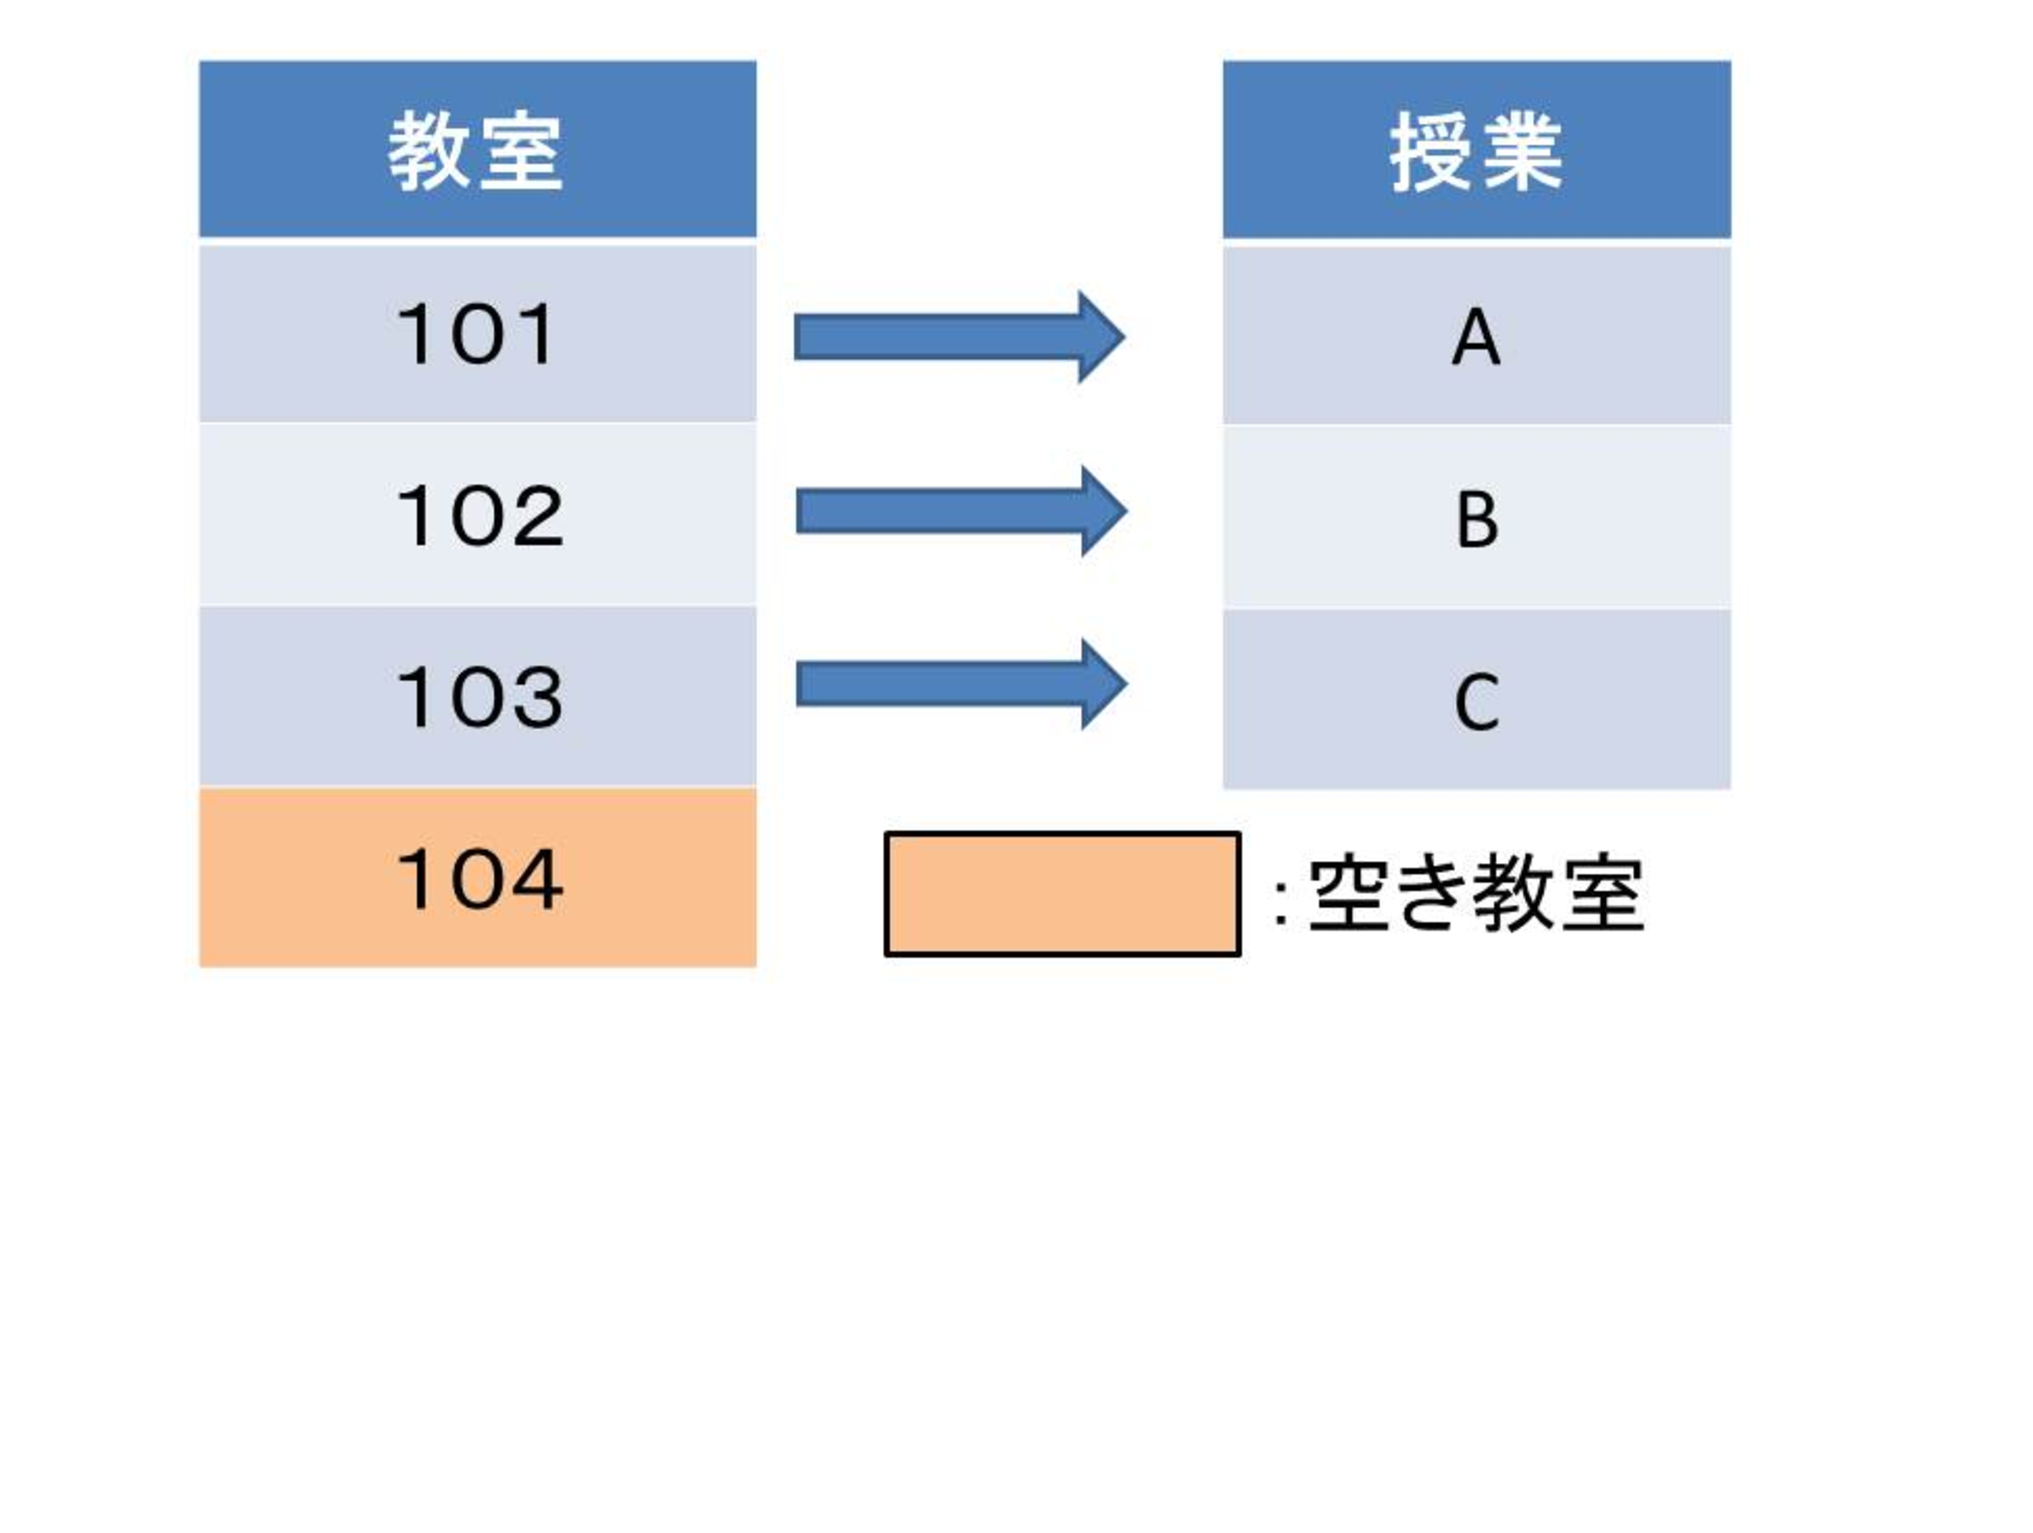
\includegraphics[width=100mm]{soturon_pre5.eps}
 \end{center}
\end{figure}


\end{frame}


\begin{frame}
 \frametitle{\LARGE 考慮制約の例}

\fbox{ 
\begin{tabular}{ll}
{\Large 考慮制約1}
\end{tabular}
}\\
\begin{center}
{\Large $u_{i1,j1}$ + $u_{i2,,j2}$ ー $1$ $\leq$ $\alpha_{j1,j2}$}\\
\vspace{2.0mm}
{\Large ($i_1,i_2 \in I,(j_1,j_2) \in L \subseteq J \times J,i_1 \neq i_2$)}
\vspace{0mm}
\begin{figure}[htbp]
 \begin{center}
  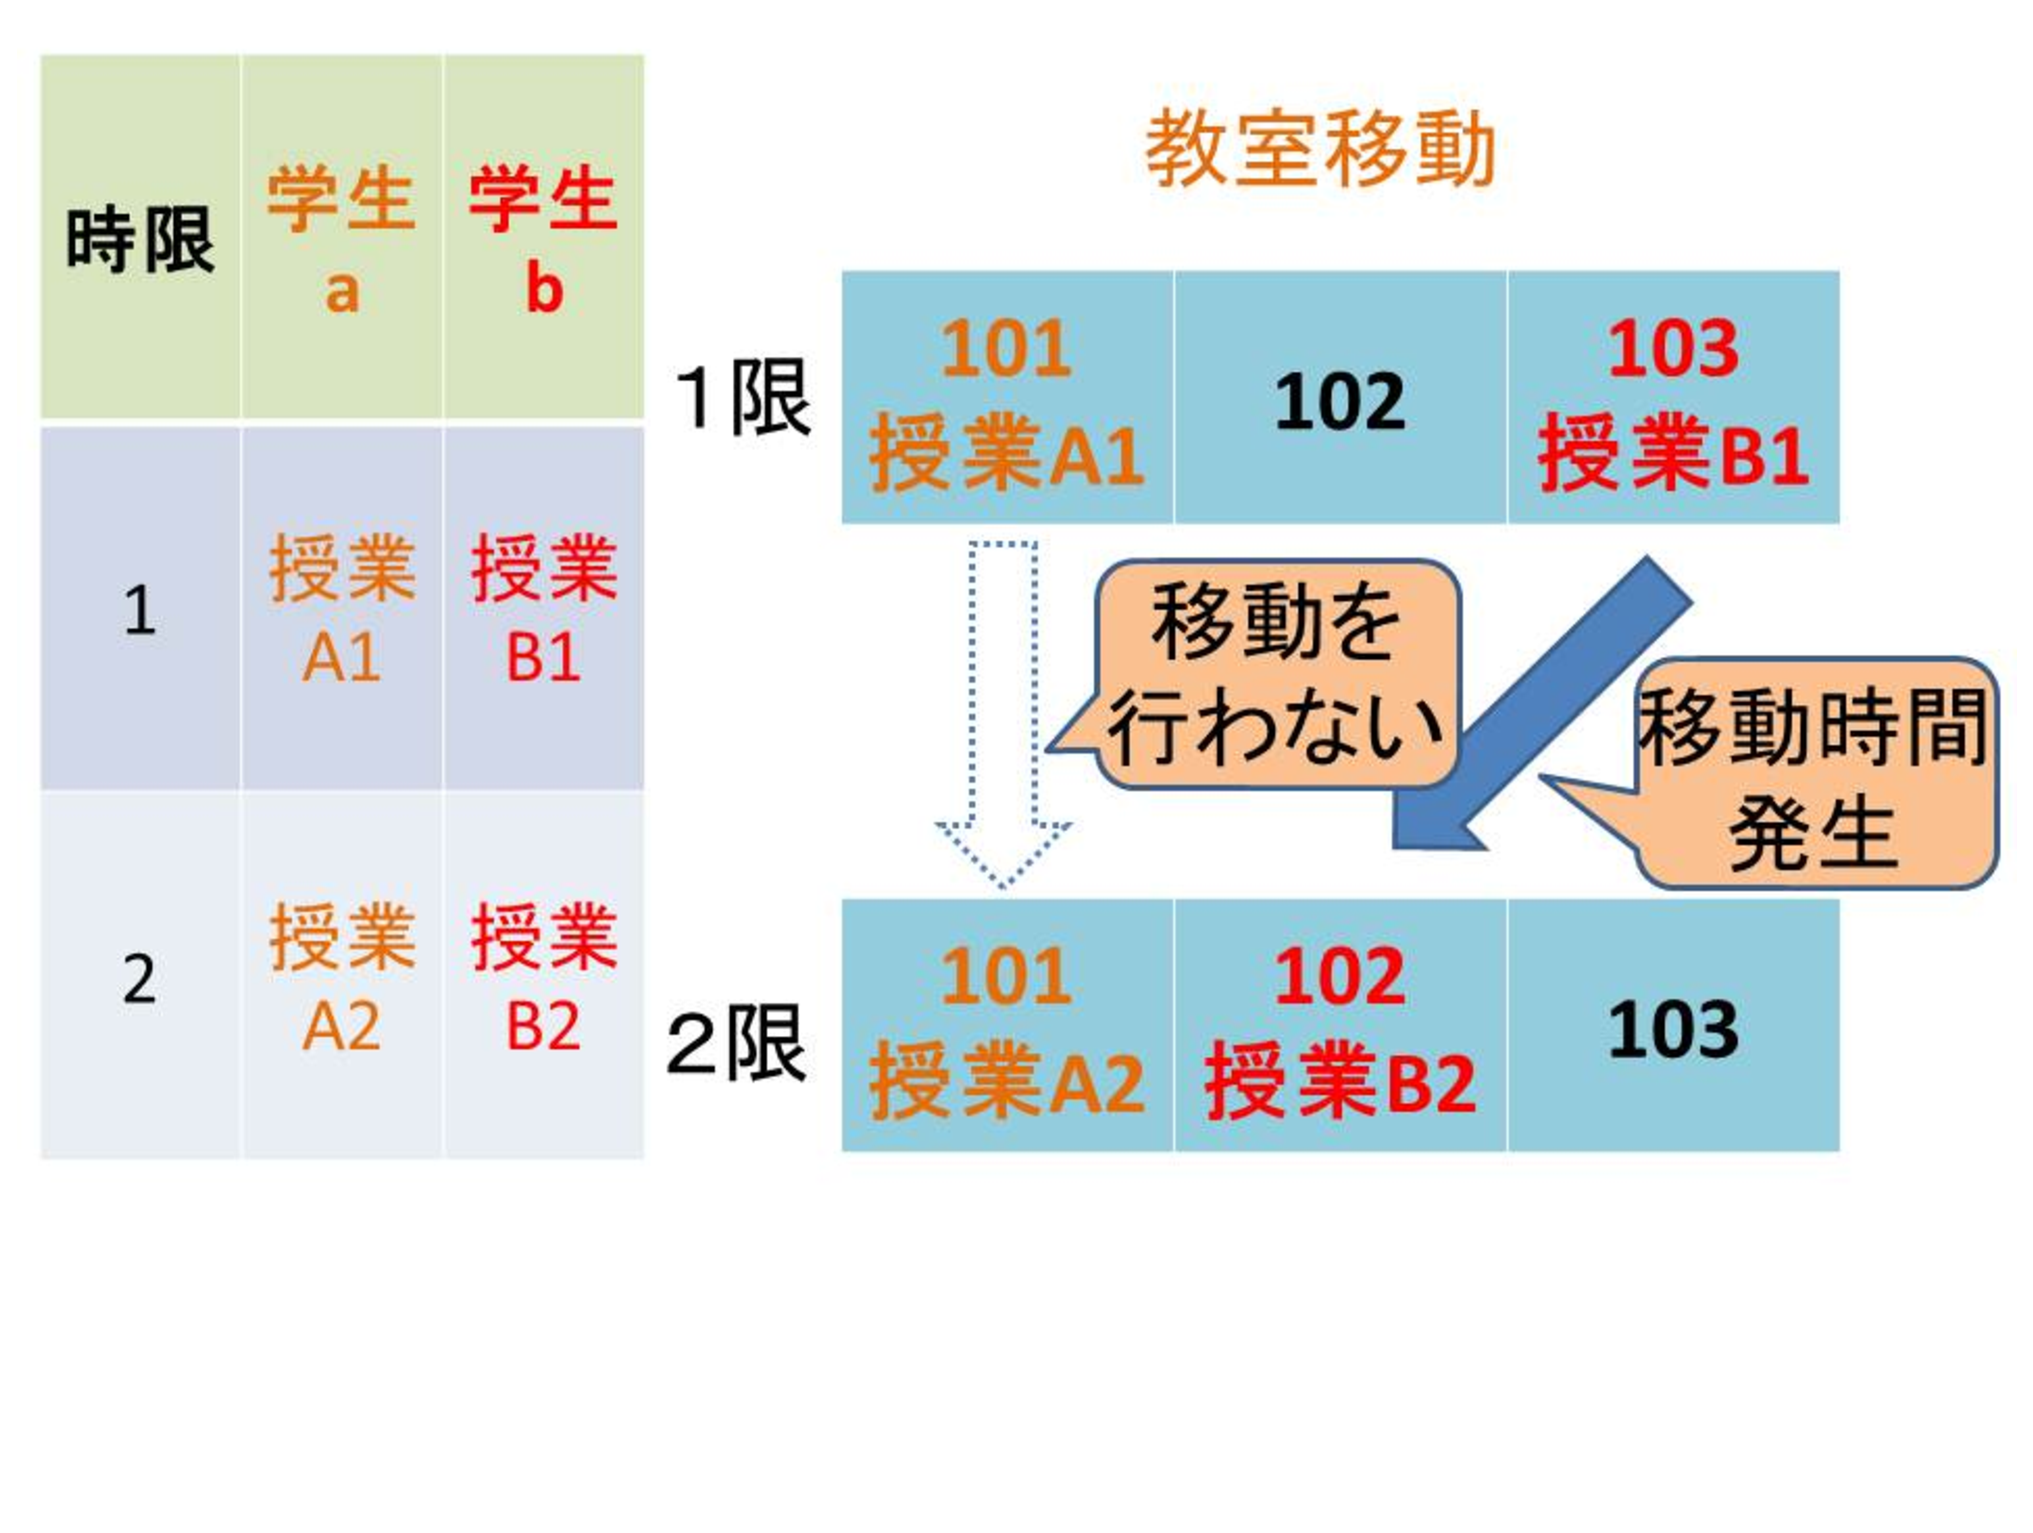
\includegraphics[width=100mm]{soturon_pre8.eps}
 \end{center}

\end{figure}
\end{center}
\end{frame}



\if0

\begin{frame}
  \frametitle{\LARGE 考慮制約}

\end{frame}
\begin{frame}
\fbox{ 
\begin{tabular}{ll}
 {\LARGE 移動時に起こる混雑の緩和}
\end{tabular}
}
\vspace{5.0mm}
\begin{figure}[htbp]
 \begin{center}
  \includegraphics[width=100mm]{tyuukan_picture9.eps}
 \end{center}
\end{figure}
\end{frame}
\fi

\begin{frame}
\frametitle{\LARGE{実験内容}}
%\begin{itemize}
%\item{\Large{実験}}
%\begin{enumerate}
%\item {\large 各データに対して計算時間の上限を1時間として行う数値計算}
%\item {\large 各データのうち,午前なら1限目,午後なら3限目の授業の中で受講者数が多い上位5つの授業の開講される教室を指定し,計算時間の上限を1時間として行う数値計算}
%\end{enumerate}
%\end{itemize}
\fbox{
\begin{tabular}{l|l}
{\Large \hspace{-3.0mm}実験1}

& {\Large \hspace{0mm}・計算時間上限:1時間  }\\
%& {\Large \hspace{0mm}として行う数値計算}\\
\end{tabular}
}
\begin{itemize}
\item{\large{実験1の目的:}}
\begin{itemize}
\item{\large{平成25年度の教室割当より移動時間の短い解が得られるか確認}}
\end{itemize}
\end{itemize}
\fbox{
\begin{tabular}{l|l}
{\Large \hspace{-3.0mm}実験2}
& {\Large \hspace{0mm}・計算時間上限:1時間  }\\
& {\Large \hspace{0mm}・教室指定:5教室  }\\
& {\Large \hspace{3mm}(受講者数が多い上位5つ)}\\
%& {\Large \hspace{0mm}多い上位5つ}\\
%& {\Large \hspace{0mm}各データのうち,授業の中で受講者数が}\\
%& {\Large \hspace{0mm}多い上位5つの授業の開講される教室を}\\
%& {\Large \hspace{0mm}指定し,計算時間の上限を1時間として}\\
%& {\Large \hspace{0mm}行う数値計算}\\
\end{tabular}
}

\begin{itemize}
\item{\large{実験2の目的:}}
\begin{itemize}
\item{\large{教室割当を指定することで変化する解と計算時間の確認}}
\end{itemize}
\end{itemize}
%\begin{table}[htb]
%\caption{計算環境}
%\scalebox{1.0}{ 
%\begin{tabular}{cc}
%\hline
%OS & Microsoft Windows 7 Service Pack 1\\
%CPU &{\small Intel(R) Core(TM) i7-3930K CPU @ 3.20GHz}\\ 
%メモリ & 32.0GB\\
%システム & 64ビット オぺレーティング システム\\
%ソルバー &IBM ILOG CPLEX 12.4.0.0\\
%\hline
%\end{tabular}
%}
%\end{table}
\end{frame}


\begin{frame}
 \frametitle{\LARGE 実験の結果}
実際にH25年度に関西大学で使用されていたデータと教室割当の結果を用いて計算を行った.
%\vspace{-2.0mm}
\begin{table}[htb]
\begin{center}
\caption{秋学期金曜日のデータを用いた実験の結果}
%\vspace{-4.0mm}
\scalebox{0.9}{ 
\begin{tabular}{lrrrrr}
\hline 
 &  & 制約 & 変数   & 目的関数値  & 計算時間(秒)\\
\hline\hline
H25年度 & 午前 & 2589008 & 6613 &  39787 & \\
H25年度 & 午後 & 42784982 & 42410 & 98523 & \\
\hline
実験1 & 午前 & 5621770 & 10224 & 1729 & 167.65\\
実験1 & 午後 & 45746441 & 45004 & 47043 & 3600.97\\
実験2 & 午前 & 5621722 & 10171 & 4145 & 17.19\\
実験2 & 午後 & 45746364 & 44922 & 24440 & 3600.91\\
\hline
 \end{tabular}
}
%\label{tb:2}
\end{center}
\end{table}
計算方法:汎用ソルバーCPLEXの分枝限定法
\end{frame}

\begin{frame}
 \frametitle{\LARGE 移動時間の変化}
\begin{figure}[htpb]
 \begin{center}
  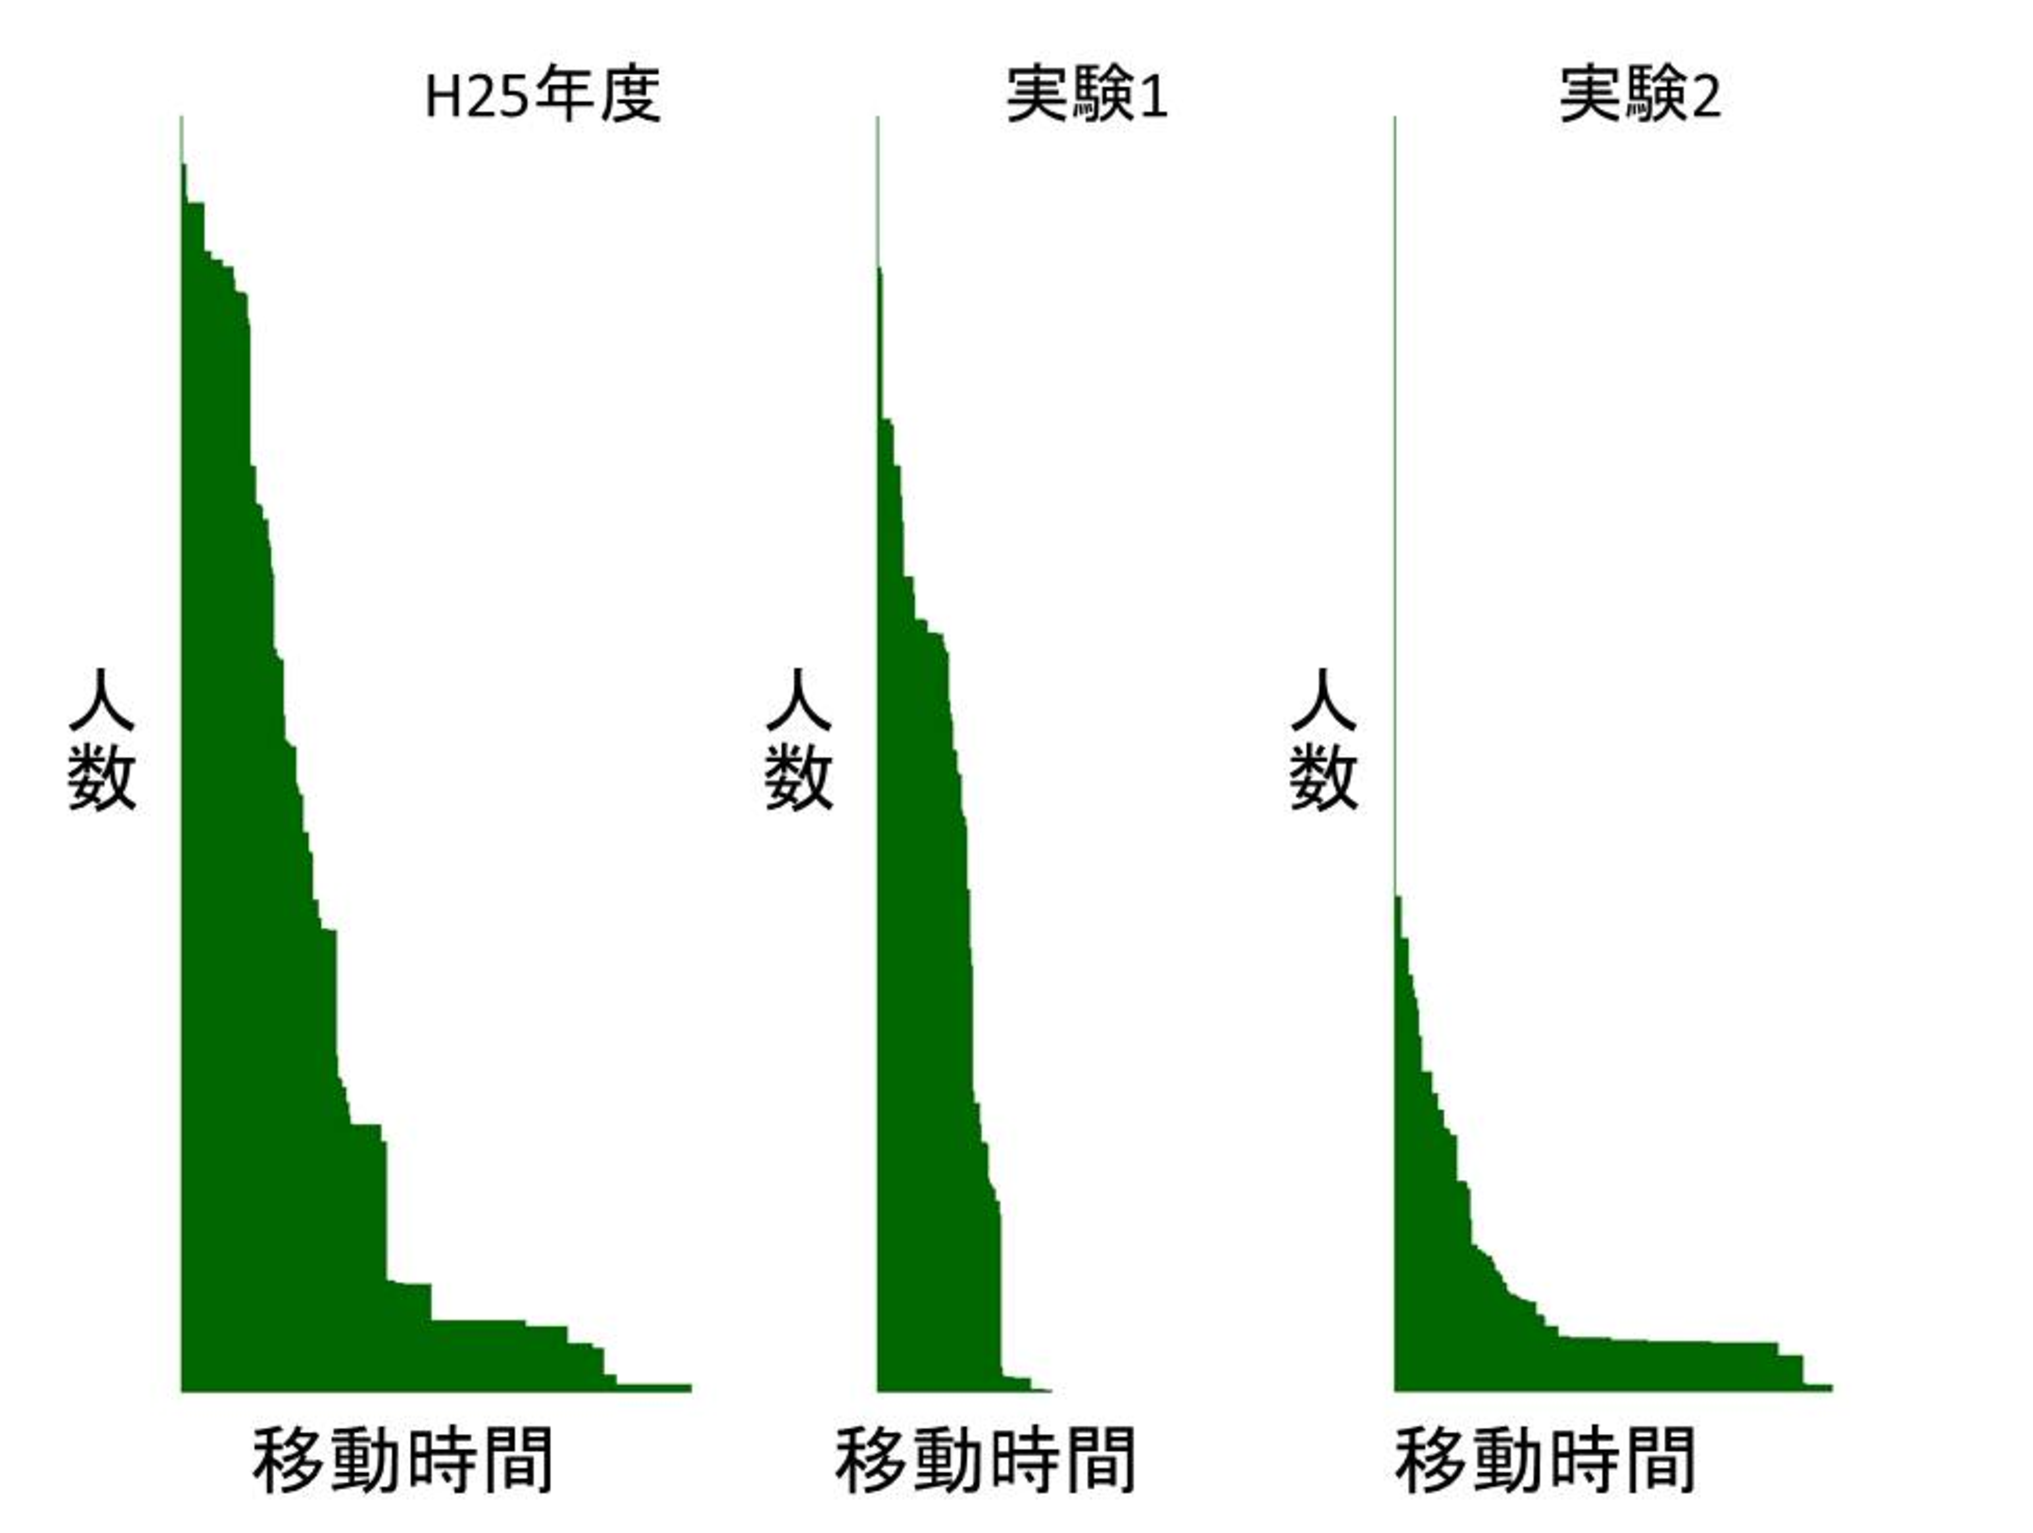
\includegraphics[scale=0.25]{giyou_picture1.eps}
\vspace{-2.0mm}
  \caption{移動時間の変化}
  \label{fig:1}
 \end{center}
\end{figure}
\end{frame}

\begin{frame}
 \frametitle{\LARGE まとめと今後の課題}
\fbox{ 
\begin{tabular}{ll}
{\LARGE まとめ}
\end{tabular}
}
\begin{itemize}
  \item {\Large 移動時間を最小化する教室割当問題の定式化を行った}
  \item {\Large H25年度の関西大学の教室割当より移動時間が短縮された教室割当を求められた}
\end{itemize}

\fbox{ 
\begin{tabular}{ll}
{\LARGE 今後の課題}
\end{tabular}
}

\begin{itemize}
  \item {\Large 混雑の発生を避ける制約の改良}
  \item {\Large 他の解法を用いた実験}
\end{itemize}
\end{frame}


\appendix





\begin{frame}
 \frametitle{\LARGE 予備実験}
\begin{center}
\large{春学期月曜午前の実データを用いた数値計算}\\
\end{center}
%目的:最適解が得られるまでに要する時間の確認\\
\begin{table}[htbp]
\begin{center}
\caption{得られた実行可能解の時間推移}
\scalebox{0.9}{ 
\begin{tabular}{lrrrr}
\hline 
 &  制約 & 変数   & 目的関数値  & 計算時間(秒)\\
\hline\hline
H25年度  &  &  & 115754 & \\
\hline
予備実験 & 269396 & 8212 & 41407 & 0.42\\
 &  &  & 9808 & 3702.22\\
 &  &  & 9032 & 7296.31\\
 &  &  & 7746 & 86461.32\\
 &  &  & 7742 & 434226.97\\
\hline
 \end{tabular}
}
\end{center}
\end{table}
\end{frame}


\begin{frame}
 \frametitle {\LARGE 集合と添字}
%\begin{itemize}
%\item {\Large 集合・添字}

\begin{itemize}
{\large
\item $p \in P$: 時限とその集合
\item $j \in J$: 授業とその集合
\item $j \in J1_p$: $p$限目に開講される授業とその集合
\item $j \in L$: 特別連続授業とその集合
\item $(i,j) \in D$: 特定の教室を指定する特定の授業の組とその集合
\item $i \in I$: 教室とその集合
}
\end{itemize}
%\end{itemize}
\end{frame}

\begin{frame}
%\begin{itemize}
\frametitle {\Large 整数パラメータ}
\[
%\hspace{-7.0mm}
\begin{array}{rcl}

b & = &
\begin{array}{ll}
\mbox{休み時間の長さ} 
\end{array}
\\




m_{i} & = & 
\begin{array}{ll}
 \mbox{教室$i$の定員数} 
\end{array}
\\


n_{j} & = & 
\begin{array}{ll}
 \mbox{授業$j$の受講者数} 
\end{array}
\\




y & = & 
\begin{array}{ll}
 \mbox{混雑が起きる可能性が高まる移動時間} 
\end{array}
\\


q_{i_1,i_2} & = & 
\begin{array}{ll}
 \mbox{授業$i_1$と授業$i_2$の双方を受講する学生数} 
\end{array}
\\


r & = & 
\begin{array}{ll}
 \mbox{全ての移動で可能な限り守りたい移動時間} 
\end{array}
\\


t_{i_1,i_2} & = & 
\begin{array}{ll}
 \mbox{教室$i_1$と教室$i_2$間での所要移動時間} 
\end{array}
\\


z & = & 
\begin{array}{ll}
 \mbox{混雑が起きると予測される人数} 
\end{array}
\\
\end{array}
\]
%\end{itemize}
\end{frame}

\begin{frame}
%\begin{itemize}
\frametitle {\Large 0-1パラメータ}
%\scalebox{0.9}{
\small{
\[
%\hspace{-7.0mm}
\begin{array}{rcl}
%\hspace{-50.0mm}
  d_{j_1,j_2} & = & \left\{ 
\begin{array}{ll}
	1, & \mbox{$p$限目に授業$j_1$を,$(p+1)$限目に授業$j_2$を受講する}\\
		& \mbox{学生が存在するとき} 		\\
	0, & \mbox{それ以外}
\end{array}
\right. \\


  e_{p,j} & = & \left\{ 
\begin{array}{ll}
	1, & \mbox{時限$p$時に授業$j$が割り当てられているとき} 		\\
	0, & \mbox{それ以外}
\end{array}
\right. \\



f_{i_1,i_2} & = & \left\{ 
\begin{array}{ll}
1, & \mbox{$t_{i_1,i_2}\leq y$であるとき} \\
0, & \mbox{それ以外}
\end{array}
\right.\\


g_{i_1,i_2} & = & \left\{ 
\begin{array}{ll}
1, & \mbox{$t_{i_1,i_2}>r$であるとき} \\
0, & \mbox{それ以外}
\end{array}
\right.\\

h_{j} & = & \left\{ 
\begin{array}{ll}
1, & \mbox{$p$限目に授業を持たず,}\\
	& \mbox{$(p+1)$限目に授業$j$を受講する学生が存在するとき} \\
0, & \mbox{それ以外}
\end{array}
\right.\\
\end{array}
\]
}
%}
%\end{itemize}
\end{frame}


\begin{frame}
 \frametitle {\LARGE 変数}
%\begin{itemize}
%\item {\Large 変数}
\small{
\[
\begin{array}{rcl}
%\hspace{-17.0mm}
v_{i_1,i_2} & = & 
\begin{array}{ll}
\mbox{ある時限に教室$i_1$で授業が開講され,}\\
\mbox{その次の時限に教室$i_2$で授業が開講されているとき,}\\
\mbox{その両方を受講している学生数}\\ 
\end{array}
\\


 u_{i,j} & = & \left\{ 
\begin{array}{ll}
1, & \mbox{教室$i$に授業$j$が割り当てられているとき} \\
0, & \mbox{それ以外}
\end{array}
\right. \\


w_{p,i_1,i_2} & = & \left\{ 
\begin{array}{ll}
1, & \mbox{$p$限目に教室$i_1$で授業が開講され,}\\
& \mbox{$(p+1)$限目に教室$i_2$で授業が開講されるとき}\\ 
0, & \mbox{それ以外}
\end{array}
\right.\\

\alpha_{j_1,j_2} & = & \left\{ 
\begin{array}{ll}
1, & \mbox{特別連続授業$j_1,j_2$が異なる教室で開講されるとき}\\
0, & \mbox{それ以外}
\end{array}
\right.\\

\beta_{j_1,j_2} & = & \left\{ 
\begin{array}{ll}
1, & \mbox{授業$j_1,j_2$間での移動時間ができるだけ守りたい指定の}\\
	& \mbox{時間を越えるとき}\\
0, & \mbox{それ以外}
\end{array}
\right.\\

\end{array}
\]
%\end{itemize}
}
\end{frame}

\begin{frame}
 \frametitle {\LARGE 変数}
%\begin{itemize}
%\item {\Large 変数}
\small{
\[
\begin{array}{rcl}

 \delta_{i,j_1,j_2} & = & \left\{ 
\begin{array}{ll}
1, & \mbox{$p$限目に授業$j$を受講していて,}\\
& \mbox{$(p+1)$限目に授業$j_2$を受講せずに}\\
& \mbox{退室する学生集団と$p$限目に授業$j_1$を受講していて,}\\
& \mbox{$(p+1)$限目に授業$j_2$を受講するために}\\
& \mbox{入室してくる学生集団か,}\\
& \mbox{$p$限目に授業を持たず$(p+1)$限目に授業$j_2$を}\\
& \mbox{受講するために入室する}\\
& \mbox{学生集団で出入りのタイミングが合い,}\\
& \mbox{混雑が起きる可能性が高いとき}\\
& \mbox{出入りのタイミングが合い,混雑が}\\
& \mbox{起きる可能性が高いとき}\\
0, & \mbox{それ以外}
\end{array}
\right.
\end{array}
\]
}
%\end{itemize}
\end{frame}


\begin{frame}

  \frametitle{\LARGE 変数を定義する制約条件}


\fbox{ 
\begin{tabular}{ll}
{\Large
$v_{i_1,i_2}$
}
\end{tabular}

}

\vspace{5.0mm}


変数$v_{i_1,i_2}$は以下の制約で定義される.

{\Large
\begin{eqnarray}
\label{eqqq:seiyaku_first} 
&&( u_{i_1,j_1} + u_{i_2,j_2} - 1 ) \cdot q_{j_1,j_2} \leq v_{i_1,i_2}\\
\nonumber\\
&&\hspace{-15.0mm} \left(\forall p \in P,\forall i_1 \in I,\forall i_2 \in I,\forall j_1 \in J1_p,\forall j_2 \in J1_{p+1},d_{j_1,j_2}=1\right)\nonumber 
\end{eqnarray}
}


\end{frame}

\begin{frame}

  \frametitle{\LARGE 変数を定義する制約条件}


\fbox{ 
\begin{tabular}{ll}
{\Large
$w_{p,i_1,i_2}$
}
\end{tabular}

}

\vspace{5.0mm}


変数$w_{p,i_1,i_2}$は以下の制約で定義される.

{\Large
\begin{eqnarray}
\label{eqneqn:seiyaku_first} 
&& u_{i1,j1} + u_{i2,j2} - 1  \leq w_{p,i_1,i_2}\\
&&\hspace{15.0mm} \left(\forall p \in P,\forall i1 \in I,\forall i2 \in I\right)\nonumber\\
&&\hspace{15.0mm} \left(\forall j1 \in J1_{p},\forall j2 \in J1_{p+1},d_{j_1,j_2}=1\right)\nonumber 
\end{eqnarray}
}


\end{frame}


\begin{frame}

  \frametitle{\LARGE 絶対制約1}



\fbox{ 
\begin{tabular}{l|l}
[絶対制約1] & 1つの曜限における各教室には2つ以上の授業を\\
&割り当てられない.\\
\end{tabular}

}
\\
\vspace{5.0mm}

本制約は,同じ曜限において,各教室に2つ以上の授業が割り当てられないようにするため,または,授業が一つも割り当てられないことを許可した制約でもある.
教室$i$について,次の制約を与える:

{\Large
\begin{eqnarray}
&&\sum_{j \in J} u_{i,j} \cdot e_{p,j} \leq 1 \hspace{5.0mm}
\quad \left (\forall p \in P, \forall i \in I \right)
\end{eqnarray} 
}
\end{frame}


\begin{frame}

  \frametitle{\LARGE 絶対制約2}


\fbox{ 
\begin{tabular}{l|l}
[絶対制約2] & 各授業には必ず1つの教室を\\
&割り当てなければならない.\\
\end{tabular}

}
\\
\vspace{5.0mm}


本制約は,ある曜限に存在する1つの授業に対して2つ以上の教室を割り当てないようにするため,または,1つの授業に1つも教室が割り当てられないことを防ぐための制約である.
授業$j$について,次の制約を与える:


{\Large
\begin{eqnarray}
&&\sum_{i \in I} u_{i,j}=1 \quad \left (\forall j \in J \right)
\end{eqnarray} 
}

\end{frame}




\begin{frame}

  \frametitle{\LARGE 絶対制約3}


\fbox{ 
\begin{tabular}{l|l}
[絶対制約3] &受講人数が教室の定員を超えて,\\
&教室に授業を割り当ててはいけない.\\
\end{tabular}

}

\vspace{5.0mm}


各教室には座席数が限られており,その数を越える受講者数を持つ授業
を割り当ててしまうと良好な状態で受講することが困難になる.
以上の状態になることを防ぐため,次の制約を与える:


{\Large
\begin{eqnarray}
&&\sum_{i \in I} u_{i,j}\cdot m_{i} \geq n_{j} \quad \left (\forall j \in J\right)
\end{eqnarray}
}
\end{frame}

\begin{frame}

  \frametitle{\LARGE 絶対制約4}


\fbox{ 
\begin{tabular}{l|l}
[絶対制約4] &特定の授業は指定された教室で\\
&開講されなければならない.\\
\end{tabular}

}

\vspace{5.0mm}


本制約は,特定の設備を必要とする授業をその設備が整った指定されている教室に割り当てるための制約である.
教室$i$に授業$j$が割り当てられなければならないとき,次の制約を与える:

{\Large
\begin{eqnarray}
&&u_{i,j}=1 \quad \left(\forall (i,j) \in D\right)
\end{eqnarray}
}
\end{frame}

\if0
\begin{frame}

  \frametitle{\LARGE 変数を定義する制約条件}


\fbox{ 
\begin{tabular}{ll}
{\Large
$v_{w,p,i_1,i_2,j_1,j_2}$
}
\end{tabular}

}

\vspace{5.0mm}


変数$v_{w,p,i_1,i_2,j_1,j_2}$は以下の制約で定義される.

{\Large
\begin{eqnarray}
&&u_{w,p,i_1,j_1}+u_{w,p+1,i_2,j_2}-1 \leq v_{w,p,i_1,i_2,j_1,j_2}\\
\label{eqn:seiyaku_first} 
&& \left(\forall w \in W,\forall p \in P\right)\nonumber 
\end{eqnarray}
}


\end{frame}




\begin{frame}

  \frametitle{\LARGE 絶対制約5}


\fbox{ 
\begin{tabular}{l|l}
[絶対制約5] &教室間の移動時間は休み時間以内でなければならない.
\end{tabular}

}

\vspace{5.0mm}

{\Large 「学生の場合」}\\
本制約は,連続する授業$j_1,j_2$が割り当てられている教室$i_1,i_2$間における移動時間が各学校の定めている休み時間を越えることを防ぐための制約である.

{\Large
\begin{eqnarray}
&&v_{w,p,i_1,i_2,j_1,j_2}\cdot d_{p,j_1,j_2}\cdot t_{i_1,i_2} \leq b 
\label{eqn:seiyaku_first} \\ 
&& \left(\forall w \in W,\forall p \in P\right)\nonumber 
\end{eqnarray}
}
{\large
($t_{i_1,i_2}$=教室$i_1$から教室$i_2$への移動時間 , $b$=休み時間)
}
\end{frame}




\begin{frame}

  \frametitle{\LARGE 絶対制約5}



\vspace{2.0mm}

{\Large 「教員の場合」}\\

遅刻の対策を考察する対象は学生のみではない,現在の授業システムでは1つの授業を開講する際,最低限1人以上の教員と1人以上の学生が必要となる.\\
本制約は,正常に授業を開講するため教員側の移動時間を考慮した制約である.\\
教員$k$が受け持つ2限連続した授業が教室$i_1,i_2$で開講されるとき,次の制約を与える.


\begin{eqnarray}
&&s_{j_1,k}\cdot s_{j_2,k}\cdot v_{w,p,i_1,i_2,j_1,j_2}\cdot t_{i_1,i_2}\leq b\\
\label{eqn:seiyaku_first} 
&& \left(\forall w \in W,\forall p \in P,\forall k \in K\right)\nonumber 
\end{eqnarray}

\end{frame}
\fi


\begin{frame}

  \frametitle{\LARGE 考慮制約1}

%\hspace{-3.0mm}
\fbox{ \hspace{-5.0mm}
\begin{tabular}{l|l}
[考慮制約1] &特別連続授業は同じ教室で開講されることが好ましい.
\end{tabular}

}

\vspace{5.0mm}


特別連続授業(授業内容が同一,または非常に関連性の高い2限連続で開講される2つの授業)は双方を受講している学生が多く,教室を移動する学生が少ないと考えられるため,そのまま同一の教室で開講されることが好ましい.
本制約は特別連続授業が別々の教室で開講されることをできるだけ防ぐための制約である.


{\Large
\begin{eqnarray}
&&u_{i_1,j_1}+ u_{i_2,j_2}- 1 \leq \alpha_{j_1,j_2} \quad \\
&&\hspace{10.0mm}\left((j_1,j_2) \in L \subseteq J \times J,i_1 \neq i_2\right)\nonumber
\end{eqnarray}
}
\end{frame}

\begin{frame}

  \frametitle{\LARGE 考慮制約2}

%\hspace{-3.0mm}
\fbox{ \hspace{-5.0mm}
\begin{tabular}{l|l}
[考慮制約2] &移動時間は指定した時間以内であることが好ましい.
\end{tabular}

}

\vspace{5.0mm}


休み時間に行うことは教室移動のみではない.前の授業の片付け,次の授業の準備などを行う必要があるため移動時間にあまり多くの時間をとられることは好ましくない.
本制約は,できるだけ休み時間を移動以外のことに費やせるようにするための制約である.


{\Large
\begin{eqnarray}
&&w_{p,i_1,i_2}\cdot g_{i_1,i_2} \leq \beta_{j_1,j_2}
\label{eqn:seiyaku_first} \\ 
&& \left(\forall p \in P,\forall i1 \in I,\forall i2 \in I,\forall j1 \in J1_p,\forall j2 \in J1_{p+1}\right)\nonumber 
\end{eqnarray}
}
\end{frame}

\begin{frame}

  \frametitle{\LARGE 考慮制約3}

%\hspace{-3.0mm}
\fbox{ \hspace{-5.0mm}
\begin{tabular}{l|l}
[考慮制約3] &教室内の人が入れ替わる際の混雑ができるだけ\\
&発生しないほうが好ましい.
\end{tabular}

}

\vspace{5.0mm}


移動が行われる教室間の距離が短い場合,移動して教室に入ってくる学生と,授業が終わって教室から出て行く学生の間で混雑が起きる.このような混雑は移動時間の増加につながるためできるだけ避けたいことである.
本制約は以上のような混雑による移動時間の増加をできるだけ避けるための制約である.

\end{frame}
\begin{frame}

  \frametitle{\LARGE 考慮制約3}
\vspace{-10.0mm}
{\Large
\begin{eqnarray}
&&((n_{j}-q_{j,j_2}\cdot d_{j,j_2}) + (q_{j_1,j_2} \cdot d_{j_1,j_2} \cdot f_{i_2,i_1}) \nonumber \\
&&+ (n_{j_2} - q_{j_1,j_2}) \cdot h_{j_2}) \cdot (u_{i_1,j} + u_{i_1,j_2} + u_{i_2,j_1} - 2) \nonumber\\
&& \cdot \ d_{j_1,j_2} - z \leq M \cdot \delta_{j,j_1,j_2} \\
&& \hspace{10.0mm} \left(\forall p \in P,\forall i_1 \in I,\forall i_2 \in I,\forall j \in J1_{p}\right)\nonumber\\
&& \hspace{10.0mm} \left(\forall j1 \in J1_{p},\forall j2 \in J1_{p+1},i_1 \neq i_2,j \neq j_1\right)\nonumber 
%&& \hspace{10.0mm} \left(i_1 \neq i_2,j \neq j_1\right)\nonumber
\end{eqnarray}
}
\vspace{-8.0mm}
\begin{figure}[H]
 \begin{center}
  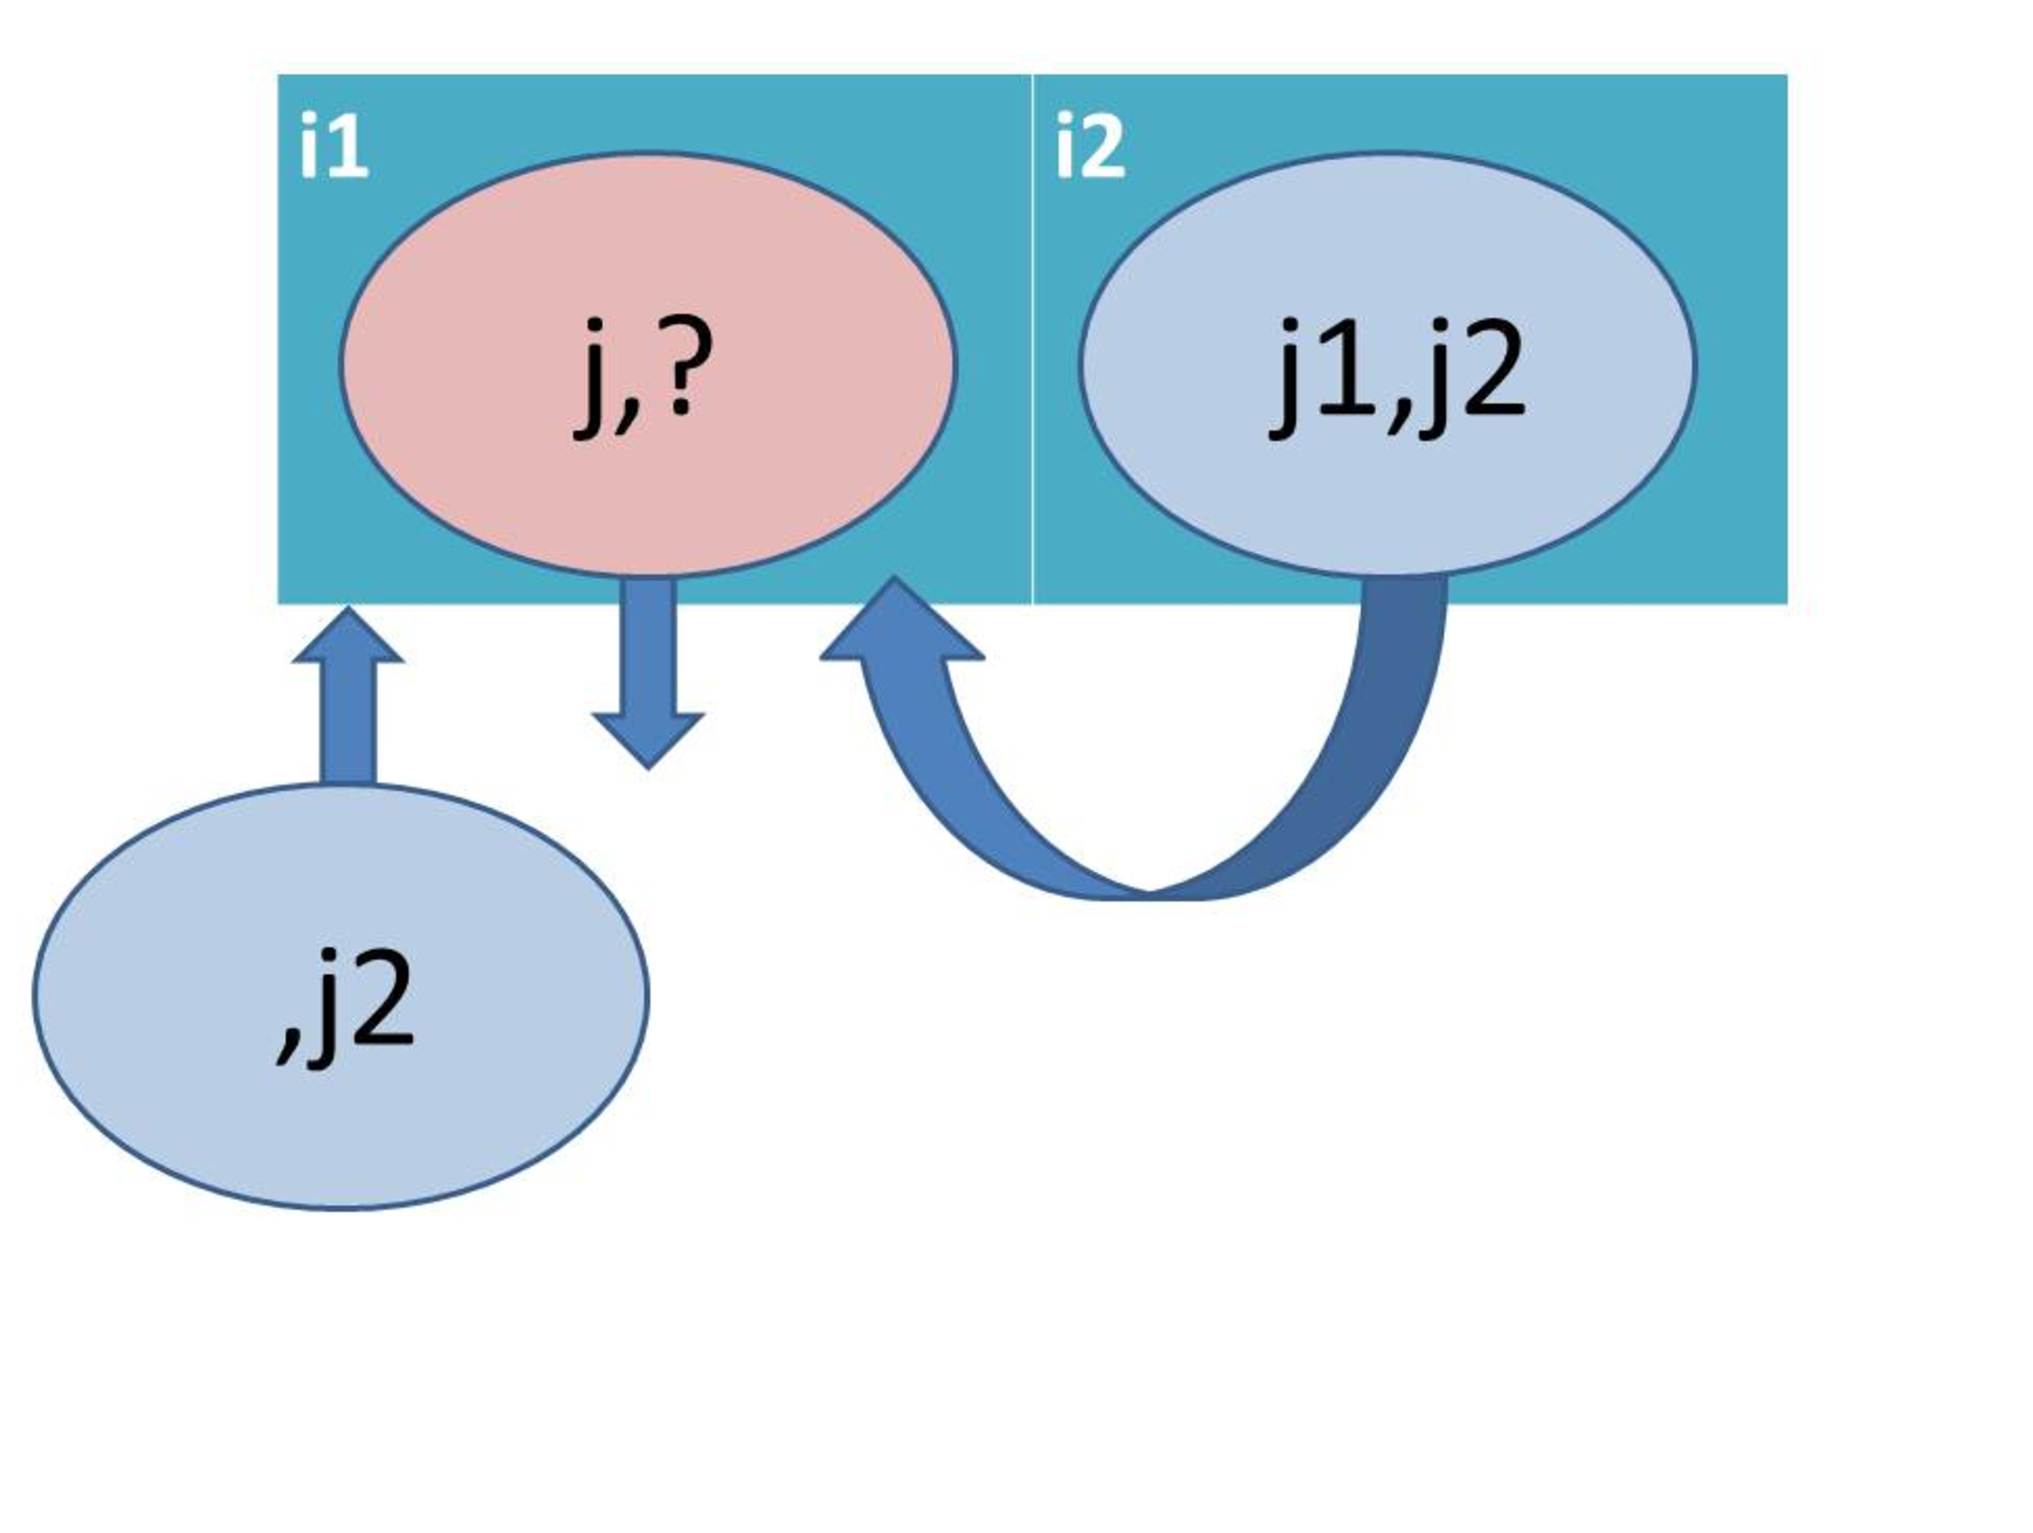
\includegraphics[width=80mm]{soturon_pre7.eps}
 \end{center}
\end{figure}
\end{frame}

\begin{frame}
\frametitle{\LARGE 違反点数}

ここでは本問題の考慮制約が満たされていない場合に発生する違反点数について記述する.\\
考慮制約1,2,3に対する違反点数$E_1,E_2,E_3$をそれぞれ(\ref{E_1}),(\ref{E_2}),(\ref{E_3})のように定める:

\begin{eqnarray}
\label{E_1}
&&E_1= \sum_{j_1,j_2 \in J}\alpha_{j_1,j_2}
\end{eqnarray}


\vspace{-5.0mm}
\begin{eqnarray}
\label{E_2}
&&E_2= \sum_{p \in P}\sum_{j_1 \in J1_{p}}\sum_{j_2 \in J1_{p+1}}\beta_{j_1,j_2}
\end{eqnarray}


\vspace{-5.0mm}
\begin{eqnarray}
\label{E_3}
&&E_3= \sum_{p \in P}\sum_{j,j_1 \in J1_{p}}\sum_{j_2 \in J1_{p+1}}\delta_{j,j_1,j_2}
\end{eqnarray}
\end{frame}

\begin{frame}
\frametitle{ \LARGE 目的関数}


目的関数は,移動を行う全学生の移動時間の総和と考慮制約を満たせていない場合に発生する違反点数$E_i(i=1,2,3)$にそれぞれの重み係数$a$と$c_i(i=1,2,3)$を掛け合わせ,それらを足した値を最小化するように定める.\\


\begin{eqnarray}
&&{\rm minimize} \quad( a \cdot \sum_{i_1 \in I} \sum_{i_2 \in I} (t_{i_1,i_2} \cdot v_{i_1,i_2})) + \sum_{i=1}^{3} c_{i} \cdot E_{i}
\end{eqnarray}
\end{frame}

\begin{frame}\frametitle{教室割当問題 \ (2013,鈴木)}
\begin{itemize}
\item 教室割当\\
\vspace{5pt}
各授業をどの教室に割り当てるか\\
(現在手動で行われている)\\
\item 教室割当問題\\
\vspace{5pt}
授業間の教室移動時間が最小となる教室割当を求める問題\\
(1,2限と3,4,5限はそれぞれ連動している.昼休みは十分に移動の時間があるため,混雑は起きないとする)

\begin{itembox}{先行研究}
数理計画問題として定式化・求解
\end{itembox}
\end{itemize}
\end{frame}



\begin{frame}\frametitle{本研究の目標}
\begin{itemize}
\item 先行研究
\begin{itemize}
\item 計算時間が長く,厳密解が得られない\\
\item 制約式に改良点が存在\\
\item 無駄な変数がある\\
\end{itemize}
\vspace{-10pt}

\begin{table}
\begin{center}
\caption{厳密解を求めることができた計算パターン}
\vspace{-5pt}
\begin{tabular}{cc|cccccc}\hline
$~$&$~$&月&火&水&木&金&土 \\ \hline
春&1,2限&$\times$&$\times$&$\times$&$\bigcirc$&$\bigcirc$&$\bigcirc$ \\ 
$~$&3,4,5限&$\times$&$\times$&$\times$&$\times$&$\times$&$\bigcirc$ \\ \hline
秋&1,2限&$\times$&$\times$&$\times$&$\times$&$\times$&$\bigcirc$ \\ 
$~$&3,4,5限&$\times$&$\times$&$\times$&$\times$&$\times$&$\bigcirc$ \\ \hline
\multicolumn{8}{c}{連動している24パターンについて計算}\\
\end{tabular}
\end{center}
\end{table}

\item 本研究
\begin{itemize}
\item 制約条件の改良・追加
\item 求解を行うインターフェイスの開発・実装
\end{itemize}

\end{itemize}

\end{frame}



\begin{frame}\frametitle{先行研究での制約条件・目的関数}
\begin{itemize}
\item 絶対制約(必ず守らなければならない制約)
\begin{itemize}
\item 1つの曜限における各教室には授業を1つしか割り当てられない
\item 各授業には必ず1つの教室を割り当てなければならない
\item 受講人数が教室の定員を超える授業を教室に割り当てられない
\item 特定の授業は指定された教室で開講されなければならない
\end{itemize}


\item 考慮制約(できるだけ守りたい制約)

\begin{itemize}
\item 特別連続授業は同じ教室で開講されることが好ましい
\item 移動時間は指定した時間以内であることが好ましい
\item 教室内の人が入れ替わる際の混雑が発生しないほうが好ましい
\end{itemize}
\item 目的関数\\
移動を行う全学生の移動時間の総和と,考慮制約を満たせて\\いない場合に発生する違反点数の合計を最小化
\end{itemize}
\end{frame}


\begin{frame}\frametitle{制約条件・目的関数}
\begin{itemize}
\item 絶対制約(必ず守らなければならない制約)
\begin{itemize}
\item 1つの曜限における各教室には授業を1つしか割り当てられない
\item 各授業には必ず1つの教室を割り当てなければならない
\item 受講人数が教室の定員を超える授業を教室に割り当てられない
\item 特定の授業は指定された教室で開講されなければならない
\item 一般授業は特殊教室で開講されてはいけない
\item 特別連続授業は同じ教室で開講されることが好ましい
\item 移動時間は指定した時間以内であることが好ましい
\end{itemize}


\item 考慮制約(できるだけ守りたい制約)

\begin{itemize}
\item 教室内の人が入れ替わる際の混雑が発生しないほうが好ましい
\item 希望教室があれば,その教室で授業を開講したい
\end{itemize}
\item 目的関数\\
混雑が発生した場合の違反点数から,希望教室を満たした場合点数の合計を最小化()
\end{itemize}
\end{frame}


\begin{frame}\frametitle{改良点1}
\begin{itembox}[l]{考慮制約1 \ (先行研究)}
特別連続授業は同じ教室で開講されることが好ましい
\vspace{-10pt}
\[u_{i_1,j_1} + u_{i_2,j_2} -1\le \alpha_{j_1,j_2} 
\quad ((j_1,j_2) \in L ,i_1 \neq i_2)\]

\end{itembox}
\vspace{-15pt}
\[
u_{i,j} = \left\{
\begin{array}{ll}
1,& \text{教室$i$で授業$j$が開講されるとき} \hspace{30pt}\alpha\text{ :違反の指標}\\
0, & \text{それ以外} \hspace{120pt} L \text{:特別連続授業の集合 }
\end{array}
\right.
\]
 

\begin{itemize}
\item 特別連続授業(関連性の高い連続で開講される2つの授業):\\ほとんどの学生が連続受講\\
\item 教室移動すると混雑の可能性大\\
\item \textcolor{blue}{絶対制約にすることで混雑発生の可能性がなくなる}\\
\end{itemize}
\begin{block}{特別連続授業は同じ教室で開講しなければならない}
\vspace{-5pt}
\[ u_{i,j_1} = u_{i,j_2} \qquad ((j_1,j_2) \in L) \]
\end{block}

\end{frame}



\begin{frame}\frametitle{改良点2}
\vspace{-6pt}
\begin{itembox}[l]{考慮制約2 \ (先行研究)}
\vspace{-5pt}
 移動時間は指定した時間以内であることが好ましい\\
\vspace{-15pt}
\[w_{p,i_1,i_2}\cdot g_{i_1,i_2} \leq \beta_{j_1,j_2}\] \\
\vspace{-0.5in}
\end{itembox}
\begin{itemize}
\vspace{-5pt}
\item 制約式が正しくない\\

\item 休み時間は必ず一定時間以上ほしい\\
絶対制約にすることで確保する
\begin{block}{移動時間は指定した時間以内でなければならない}
教室$i_1$,$i_2$間で移動する学生の移動時間が指定した時間を越える場合,
\vspace{-10pt}
\[ u_{i_1,j_1}+u_{i_2,j_2}\le 1\]\\

\end{block}
\end{itemize}
\end{frame}




\begin{frame}\frametitle{改良点3-1}
\begin{itembox}[l]{考慮制約3 \ (先行研究)}
教室内の人が入れ替わる際の混雑が発生しないほうが好ましい\\
\vspace{-15pt}
\end{itembox}
\vspace{-15pt}
\begin{itemize}
\item 先行研究 :遠くの教室から来る人は混雑の対象とならない\\
\item 本研究:教室を出入りするすべての人が混雑の対象\\
(遠くの教室が早く授業終了,対象教室の授業終了が遅れるなど)\\
\begin{figure}

		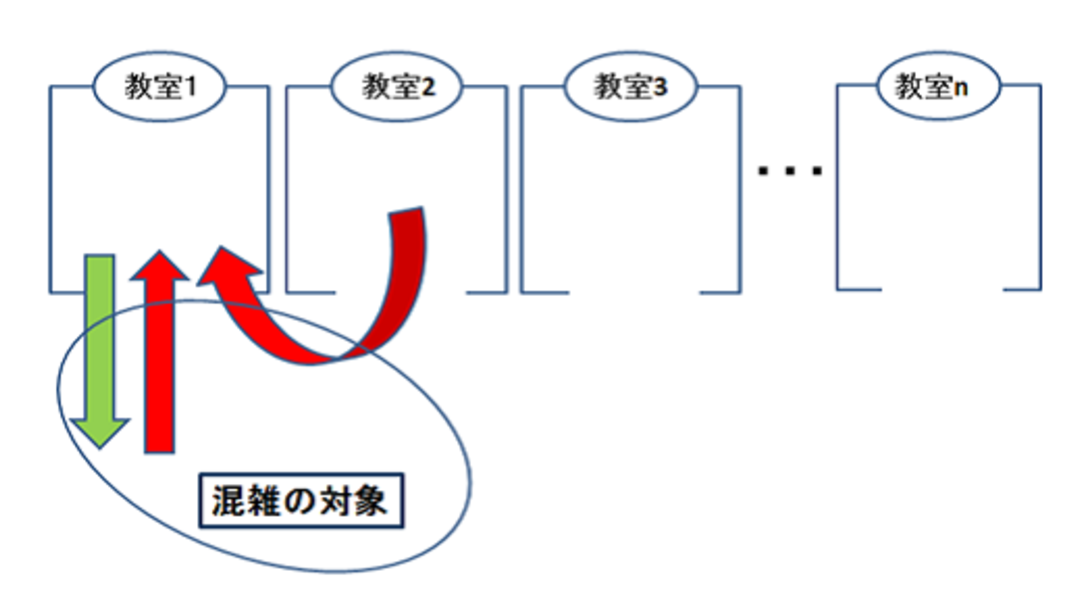
\includegraphics[width=7cm]{kouryo3_old8.eps}
	
\end{figure}
\end{itemize}
\end{frame}

\begin{frame}\frametitle{改良点3-2}
\begin{itembox}[l]{考慮制約3 \ (先行研究)}
教室内の人が入れ替わる際の混雑が発生しないほうが好ましい\\
\vspace{-15pt}
\end{itembox}
\vspace{-15pt}
\begin{itemize}
\item 先行研究 :遠くの教室から来る人は混雑の対象とならない\\
\item \textcolor{blue}{本研究:教室を出入りするすべての人が混雑の対象}\\
(遠くの教室が早く授業終了,対象教室の授業終了が遅れるなど)\\

\begin{figure}

		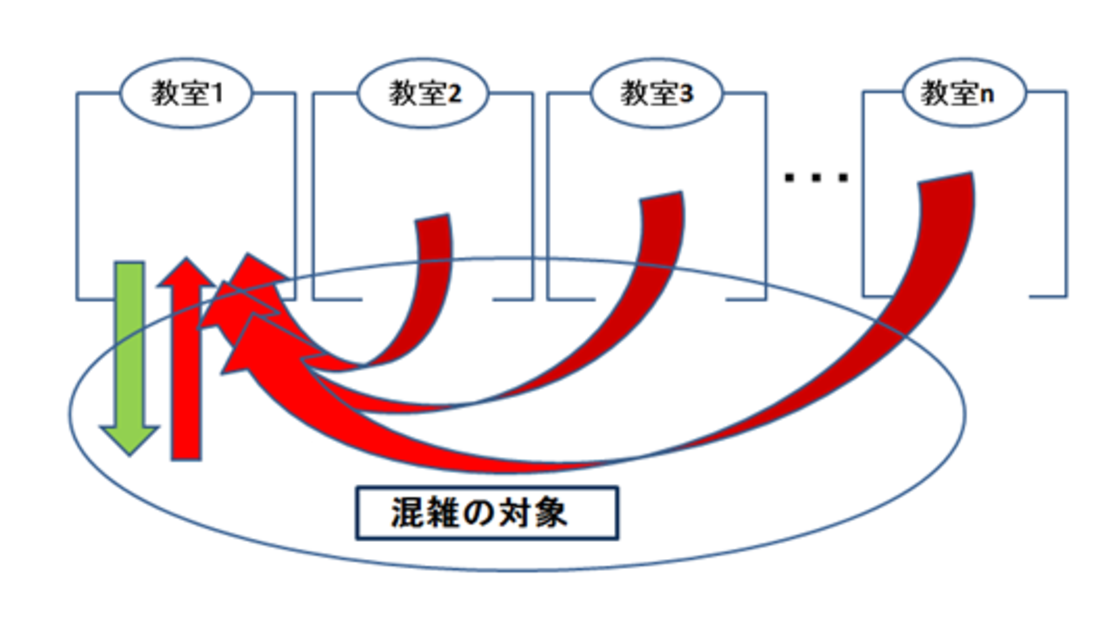
\includegraphics[width=7cm]{kouryo3_new8.eps}
	
\end{figure}
\end{itemize}
\end{frame}


\begin{frame}\frametitle{追加する制約条件}
\begin{itemize}

\item 授業$j$に対する希望教室がある \\
研究室と近いetc...\\
\item 絶対制約にすると\\
希望が重なるかもしれないので向いていない\\
\item 考慮制約にする

\begin{block}{授業$j$を希望教室で開講したい}
\[\text{違反点数} = \gamma \sum_j\sum_{i \in I \setminus I_j}u_{i,j} \]
\qquad \qquad ($I$:全教室の集合,$I_j$:授業$j$の希望教室の集合)
\end{block}
各授業を希望した教室で開講できない場合,目的関数に違反点数を加算

\end{itemize}
\end{frame}



\begin{frame}\frametitle{まとめと今後の予定}
\begin{itembox}[l]{まとめ}
\begin{itemize}
\vspace{-5pt}
\item 先行研究の勉強
\item 制約条件の改良・追加
\vspace{-5pt}
\end{itemize}
\end{itembox}
\begin{itembox}[l]{今後の予定}
\vspace{-5pt}
\begin{itemize}
\item 9月\\
\begin{itemize}
\item モデルファイルの作成
\end{itemize}
\item 10月\\
\begin{itemize}
\item 第4学舎のデータを用意  (授業情報,教室間の移動時間...)
\item ソルバーを選定し,計算する		
\end{itemize}
\item11月~\\
\begin{itemize}
\item 求解を行うインターフェイスの開発・実装
\end{itemize}
\vspace{-5pt}
\end{itemize}
\end{itembox}

\end{frame}

\end{document}
